% Op icon: boolean union — two overlapping circles, both filled solid.
\documentclass[tikz,border=2mm]{standalone}
\usetikzlibrary{arrows.meta,calc,shapes.geometric}
\begin{document}
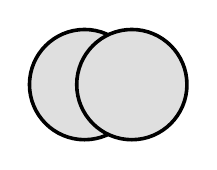
\begin{tikzpicture}[line width=1.3pt, line cap=round, line join=round, >=Stealth, x=1mm,y=1mm]
  \filldraw[fill=gray!25] (-3,0) circle (7);
  \filldraw[fill=gray!25] (3,0) circle (7);
\end{tikzpicture}
\end{document}
